\textbf{1-1} 【题1】道尔顿提出过一种定压温标。在此温标下，压强为一恒定值时，理想气体体积的相对增量正比于温度 $\tau$ 的增量，且也将冰点定为 $\tau = 0^{\circ}$ ，汽点定为 $\tau = 100^{\circ}$ 。试用摄氏温度 $t$ 来表示道尔顿温度 $\tau$ 。
\vfill

\textbf{1-2} 【题2】某热电偶测温计的一个触点始终保持为 $0^{\circ}\mathrm{C}$ ，另一触点与待测温度的物体接触。当待测温度为 $t^{\circ}\mathrm{C}$ 时，测温计中的热电动势为
$$
\mathcal {E} = \alpha t + \beta t ^ {2}
$$
其中 $\alpha = 0.20\mathrm{mV} / \mathrm{C},\beta = -5.0\times 10^{-4}\mathrm{mV} / (\mathrm{C})^2.$

如果以热电偶的热电动热 $\varepsilon$ 为测温属性，规定下述线性关系来定义温标 $t^{*}$ ：
$$
t ^ {*} = a \mathcal {E} + b
$$

并规定冰点的 $t^* = 0^\circ$ ，汽点的 $t^* = 100^\circ$ .试画出 $t^{*}(t)$ 曲线.
\vfill

\newpage
\textbf{1-3} 【题3】贮气罐的体积为 $V$ ，罐内气体压强为 $p$ 。贮气罐经阀门与体积为 $V_0$ 的真空室相连，打开阀门，为真空室充气，达到平衡后，关闭阀门；然后换一个新的同样的贮气罐继续为真空室（已非“真空”）充气；…。如此不断充气，直到真空室中气体的压强达到 $p_0 (p_0 < p)$ 为止。设充气过程中温度恒定不变。试问共需多少个贮气罐。
\vfill

\textbf{1-4} 【题4】如热图1-4-1，在地面上竖直放置一个截面均匀的 $U$ 型管，管内盛有水。如热图1-4-1所示，管的右上端开口，左上端封口，左侧水面与上端相距 $h_1 = 30\mathrm{cm}$ ，其间封有一定质量的理想气体，右侧水面与上端相距 $h_2 = 20\mathrm{cm}$ 。在右侧水面上放置一个质量可忽略不计的薄活塞，它与管壁间既无空隙又无摩擦。当从右侧上端缓慢注入高为 $H = 7.5\mathrm{cm}$ 的水银柱时，发现水银柱的上表面恰好与左侧水面等高。设注入水银过程中，环境温度与空气压强均不变。已知水银密度是水密度的13.6倍。试求空气压强 $p_0$ 的大小
\begin{center}
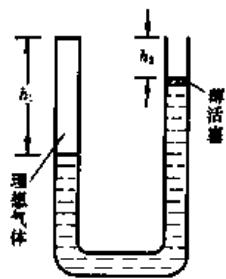
\includegraphics[width=0.2\textwidth]{figures/热图1-4-1.jpg}
\end{center}
\vfill

\newpage
\textbf{1-5} 【题5】在一端封闭、一端开口、内径均匀的直玻璃管内，有一段 $60\mathrm{mm}$ 长的水银柱。当管水平

放置达到平衡时, 闭端 A 管内空气柱长 140 mm, 开端 B 管内空气柱长也为 140 mm, 如热图 1-5-1 所示. 今将此管轻轻倒转, 使开口向下, 然后再竖直地插入水银槽内, 达到平衡时管中闭端 A 管内空气柱长 133 mm, 设大气压强为 760 mmHg, 温度不变. 试求槽中水银进入管中的高度 H.

\begin{center}
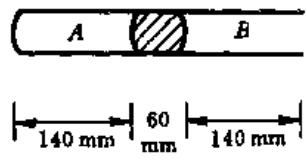
\includegraphics[width=0.25\textwidth]{figures/热图1-5-1.jpg}
\end{center}
\vfill

\textbf{1-6} 【题6】如热图1-6-1，一根均匀玻璃管长 $96\mathrm{cm}$ ，一端封闭，一端开口，竖直放置，开口端向上。管内有一

段长为 20 cm 的水银柱, 当温度为 27 ℃ 时, 水银柱下方被封闭的空气柱的长度为 60 cm, 外界的大气压强为 76 cmHg. 试问当温度升高到多少时, 水银柱刚好从管中全部溢出. 设玻璃管和水银因温度升高而产生的膨胀可忽略不计, 设外界大气压强始终保持不变, 设被封闭的空气可视为理想气体.
\begin{center}
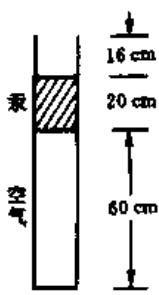
\includegraphics[width=0.3\textwidth]{figures/热图1-6-1.jpg}
\end{center}
\vfill

\newpage
\textbf{1-7} 【题7】如热图1-7-1，截面均匀，下端 $A$ 封闭的细长试管 $AB$ 竖直放置。管下端 $A$ 内封有长为 $L_{0}$ 的空气，管中间是长为 $L = 4L_{0}$ 的水银柱，管上端 $B$ 有长为 $L_{0}$ 的空气。开始时，管上端 $B$ 与大气连通，大气压强为 $p_0 = 2\rho gL$ ，其中 $\rho$ 为水银密度。

1. 如果先将 B 端封闭, 再将试管缓慢倒转 $180^{\circ}$ , 试问管中 A 端空气柱长度 $L_{A}$ 与 B 端空气柱长度 $L_{B}$ 各为多少 $L_{0}$ ?

2. 如果 $B$ 端始终与大气连通, 不封闭, 先将试管缓慢倒转 $180^{\circ}$ , 再缓慢回转 $180^{\circ}$ 复原. 试问最后管中 $A$ 端空气柱长度 $L_{A}^{\prime}$ 与 $B$ 端空气柱长度 $L_{B}^{\prime}$ 各为多少 $L_{0}$ ?

设倒转过程均在大气环境下进行,温度不变.

\begin{center}
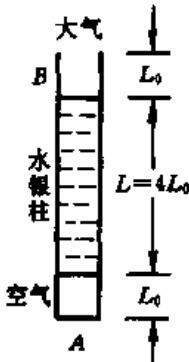
\includegraphics[width=0.15\textwidth]{figures/热图1-7-1.jpg}
\end{center}
\vfill

\textbf{1-8} 【题8】如热图1-8-1，一个装有进水孔 $a$ 和排水孔 $b$ 的铁制水箱，质量为 $840\mathrm{kg}$ ，容积为 $1\mathrm{m}^3$ 。此箱不

慎沉入湖底, 箱内充满了水, 排水孔 $b$ 与湖面相距 $10 \mathrm{~m}$ . 今采用充气法打捞水箱, 先将管子与进水孔 $u$ 连接, 用压气机把空气打进箱内, 使箱内的水排出一部分. 试问要打进多少体积的压强为 $1 \mathrm{atm}$ 、温度为 $27^{\circ} \mathrm{C}$ 的空气, 水箱才开始上浮? 设湖底的水温为 $7^{\circ} \mathrm{C}$ , 空气重量可略, 水箱铁壳的体积可略, 水的密度随湖深度的变化也可忽略.
\begin{center}
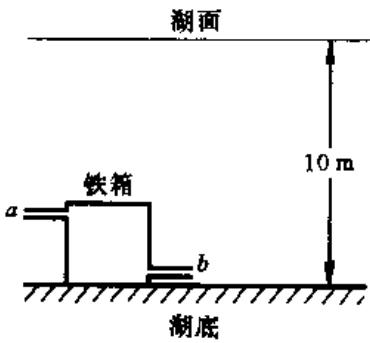
\includegraphics[width=0.25\textwidth]{figures/热图1-8-1.jpg}
\end{center}
\vfill

\newpage
\textbf{1-9} 【题9】一球形热气球,总质量(包括隔热很好的球皮以及吊篮等装载)为300 kg.经加热后,气球膨胀到最大体积,其直径为18 m.设球内外气体成份相同,球内气体压强稍高于大气压.已知大气温度为27 ℃,压强为1 atm,标准状态下空气的密度为1.3 kg/m³.试问热气球刚好能上升时,球内空气的温度应为多少?
\vfill

\textbf{1-10} 【题10】一薄壁圆柱形浮沉子一端封闭，一端开口。将开口端向下插入密度为 $\rho$ 的液体中，浮沉子内气体被封闭，当液体上方大气压强为 $p_0$ 时，闭端刚好与液面持平。若突然将液面上方压强增为 $2p_0$ ，试证明浮沉子下沉深度 $x$ 与它在该处运动速度 $v$ 的关系为

$$
v ^ {2} = 2 g x - \frac {2 p _ {0}}{\rho} \ln \left(1 + \frac {\rho g x}{2 p _ {0}}\right)
$$

其中 g 为重力加速度．设空气密度与 $\rho$ 相比可以忽略，空气可看作理想气体，不计任何粘滞阻力，且设液体内处处温度相同．
\vfill

\newpage
\textbf{1-11} 【题11】宇宙飞船投放的一个仪器以恒定速度垂直下落，接近并到达某行星的表面。该仪器用约定单位记录的压强 p 随时间 t 变化的曲线如热图1-11-1所示。落到行星表面时，该仪器还测出环境温度为 $T = 700 \, K$ ，行星表面自由落体加速度为 $g = 10 \, m/s^{2}$ 。已知该行星的大气由二氧化碳构成。试求仪器下落的速度 v。
\begin{center}
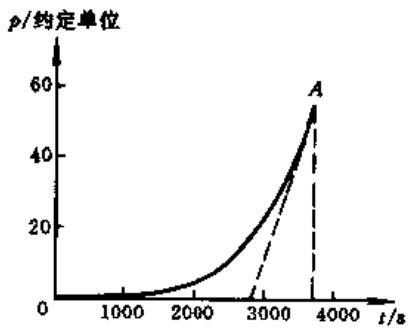
\includegraphics[width=0.25\textwidth]{figures/热图1-11-1.jpg}
\end{center}
\vfill

\textbf{1-12} 【题12】所谓某混合理想气体中各组分的体积百分比，是指各组分单独处在与混合理想气体相同压强与温度状态下，其体积在混合理想气体体积中所占的百分数。空气可当作理想气体，空气中几种主要组分的体积百分比是，氮 $(\mathbf{N}_2)78\%$ ，氧 $(\mathrm{O}_2)21\%$ ，氩（Ar） $1\%$ 。试求在标准状态(1atm, $0^{\circ}\mathrm{C}$ )下空气的密度。已知氮、氧、氩的分子量分别是28.0,32.0,39.9。
\vfill

\newpage
\textbf{1-13} 【题13】一块铝片先在干燥空气中测量质量，再在潮湿空气中测量质量。已知潮湿空气中水蒸气的分压为 $15.2\mathrm{mmHg}$ ，称质量时采用铜砝码，大气压强为 $760\mathrm{mmHg}$ ，在两种测量时温度相同为 $20^{\circ}\mathrm{C}$ 。如果所用称的灵敏度只能对 $0.1\mathrm{mg}$ 的差别才有反应，试问铝片至少应有多少质量才能在上述两种测量下表现出差别。

已知铝的密度为 $2.7 \, g/cm^{3}$ ，铜的密度为 $8.5 \, g/cm^{3}$ ， $20^{\circ}C$ 的空气的密度为 $0.0012 \, g/cm^{3}$ ，水蒸气的密度为 $0.00075 \, g/cm^{3}$ .
\vfill


\textbf{1-14}【题 14】由固态导热材料做成的长方体容器,被一隔板分成两个互不连通的部分,其中分别贮有相等质量的干燥空气和潮湿空气,在潮湿空气中水汽质量占2%.

1. 若隔板可自由无摩擦地沿器壁滑动。试求达到平衡后，干空气和湿空气所占体积的比值。

2. 若一开始采用能确保不漏气的方式将隔板抽出，试求达到平衡后容器内气体的压强，与未抽出隔板时干空气和湿空气各自的压强这三者的比值。

设干空气和湿空气均可视为理想气体。
\vfill
\newpage

\textbf{1-15}【题 15】如热图1-15-1所示,一端开口,另一端封闭的长圆柱形导热容器开口向上竖直放置.在气温为27℃,气压为760 mmHg,相对湿度(空气中水蒸气压强与该温度下饱和水蒸气压强的比值)为75%时,同一质量可忽略不计的光滑薄活塞将开口端封闭.已知水蒸气的饱和蒸汽压在27℃时为26.7 mmHg,在0℃时为4.58 mmHg.

试问:1. 若保持温度不变,通过在活塞上方注入水银增加压强的方法使管内开始有水珠出现,则容器至少应为多长?

2. 若在水蒸气刚开始凝结时固定活塞, 降低容器的温度, 则当温度降至 $0^{\circ}$ C 时, 容器内气体的压强为多大?
\begin{center}
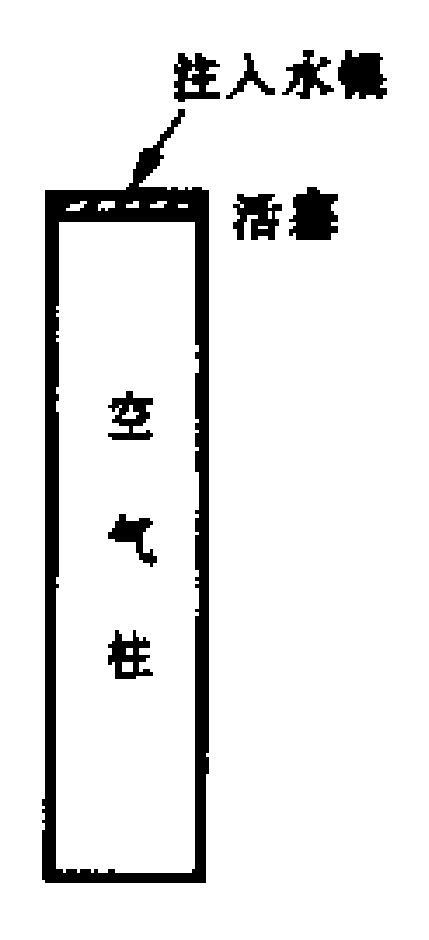
\includegraphics[width=0.08\textwidth]{figures/热图1-15-1.jpg}
\end{center}
\vfill

\textbf{1-16}【题16】如热图1-16-1，一根两端封闭、粗细均匀的石英管竖直放置，管内有一段水银柱，水银柱下方为空气，上方为一种可分解的双原子分子气体。这种双原子分子气体的性质是，当温度 $T > T_0$ 时，它的双原子分子开始分解为单原子分子。若用 $n_0$ 表示 $T_0$ 时的双原子分子数，用 $\Delta n$ 表示 $(T_0 + \Delta T)$ 时分解了的双原子分子数，则当 $\Delta T$ 很小时，分解遵循的规律为

$$
\frac {\Delta n}{n _ {0}} = \frac {\Delta T}{T _ {0}}
$$

已知初始温度为 $T_{0}$ ，此时下方空气柱的长度为 $2l_{0}$ ，上方气柱的长度为 $l_{0}$ ，水银柱产生的压强为下方空气柱压强的 $\alpha$ 倍 ( $0 < \alpha < 1$ )。设石英管和水银柱体积随温度的变化可以忽略。试问当温度由 $T_{0}$ 稍稍增加时, 水银柱将上升还是下降?

\begin{center}
    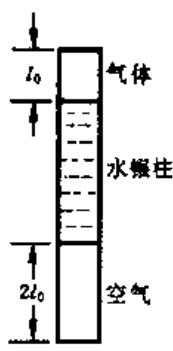
\includegraphics[width = 0.1\textwidth]{figures/热图1-16-1.jpg}
\end{center}

\vfill








